\documentclass[12pt]{article}
\usepackage[spanish]{babel}
\usepackage{graphicx}
\usepackage{amsmath}
\usepackage{amssymb}
\usepackage{cancel}
\usepackage{xcolor}
\usepackage{esint}
\usepackage{pgfplots}

\graphicspath{ {Imagenes/} }


\setlength{\parindent}{0pt}

\DeclareMathOperator{\arcsec}{arcsec}
\DeclareMathOperator{\arccot}{arccot}
\DeclareMathOperator{\arccsc}{arccsc}
\DeclareMathOperator{\di}{d\!}

\date{5 de febrero de 2021}
\title{Serie 4: Cálculo Vectorial}
\author{Ricardo López \and Dante Argüello \and Eugenio \and Ricardo Ruelas}

\begin{document}
	
\maketitle
	
\newcommand{\Int}{\int\limits}

\newcommand*\eval[3]{\left.#1\right\rvert_{#2}^{#3}}

\noindent \textbf{Ejercicio 1:} Calcular $\int_0^1 \int_0^2 xy \,dy\,dx$ .

\vspace{5mm}

\noindent \textbf{Solución.}
 
\vspace{5mm}

\begin{align*}
\int_0^1 \int_0^2 xy \,dy\,dx = \int_0^1 \eval{\frac{xy^2}{2}}{2}{0} \di x 
= \int_0^1 2x \di x 
= \color {red} 1
\end{align*}

\noindent \textbf{Ejercicio 2:} Evaluar la integral doble $\int\int_{R}x^2\sqrt{9-x^2}dA$ con R: $x^2+y^2=9$ 
\\[10pt]
\textbf{Solución.}
\\[10pt]
De $x^2+y^2=9$, $y=\sqrt{9-x^2}$ $\rightarrow$ $0\leq x\leq3$ y $0\leq y \leq\sqrt{9-x^2}$
\\[2pt]
Y para $\frac{1}{4}$ de región, la integral queda:
\[ \int_{0}^{3} \int_{0}^{\sqrt{9-x^2}}x^2\sqrt{9-x^2} \,dx\,dy \]
Entonces $I=4\int_{0}^{3} \sqrt{9-x^2}x^2\sqrt{9-x^2} \,dx=4\int_{0}^{3} 9x^2-x^4 \,dx=4(3\cdot3^3-\frac{1}{5}3^5)$
\\[4pt]
$I=4(81-\frac{243}{5}) \qquad \pmb{\color{red} \therefore \qquad I=\frac{648}{5}}$
\\[15pt]

\noindent \textbf{Ejercicio 3:} Calcular la integral doble $\int\int_{R}e^{\,x^2+y^2}dA$ donde R es la región del plano XY entre las circunferencias $x^2+y^2=9$  y $x^2+y^2=1$ 
\\[10pt]
\textbf{Solución.}
\\[10pt]
Para R: $0\leq \theta \leq2\pi$ y $\leq r \leq 3$ y con $x^2+y^2=r^2$ con $x=rcos\theta$ y $y=rsen\theta$
\\[2pt]
Entonces $dA=J(\frac{x,y}{r,\theta})=h_{r}h_{\theta}drd\theta$, $h_{r}=1$ y $h_{\theta}=r$ \hspace*{0.25cm}$\rightarrow$ \hspace*{0.25cm} $dA=rdrd\theta$
\\[2pt]
Y la integral $\int\int_{R}e^{\,x^2+y^2}dA$ quedaría como:
\[ \int_{0}^{2\pi} \int_{1}^{3}e^{\,r\cdot r} \,dr\,d\theta \]
\\[2pt]
$\int(e^{\,r\cdot r})r \,dr=\frac{1}{2}\int e^u \,du= \frac{1}{2}(e^{\,r\cdot r})$ con $u=r^2$ y $du=2dr$ $\int_{0}^{2\pi}\frac{1}{2}(e^9-e) \,d\theta \\ \\ \pmb{\color{red} \therefore \qquad \pi((e^9-e)}$
\\[15pt]

\noindent \textbf{Ejercicio 5:} Calcular el área de la región del plano XY interior a las curvas de ecuaciones $x^2+y^2=9$ y $x^2+y^2-6x=0$
\\[10pt]
\textbf{Solución.}
\\[10pt]
De la primera curva $r=3$ y de la segunda $r=6cos\theta$ Igualando $\rightarrow$ $3=6cos\theta$ y $\theta=\frac{\pi}{3}$
\\[2pt]
Entonces para $R_{1}: 0\leq \theta \leq \frac{\pi}{3}$ y $0\leq r \leq3$ y para $R_{2}: \frac{\pi}{3}\leq \theta \leq \frac{\pi}{2}$ y $0\leq r \leq6cos\theta$
\\[2pt]
Entonces la integral I=A quedaría como:
A=2(\[ \int_{0}^{\frac{\pi}{3}} \int_{0}^{3} r \,dr\,d\theta \]+\[ \int_{\frac{\pi}{3}}^{\frac{\pi}{2}} \int_{0}^{6cos\theta} r \,dr\,d\theta \])
\\[2pt]
$A=2(\int_{0}^{\frac{\pi}{3}}\rceil_{0}^{3} \frac{r^2}{2}d\theta+\int_{\frac{\pi}{3}}^{\frac{\pi}{2}}\rceil_{0}^{6cos\theta} \frac{r^2}{2}d\theta)=2(\rceil_{0}^{\frac{\pi}{3}}\frac{9}{2}\theta+\rceil_{\frac{\pi}{3}}^\frac{\pi}{2}18(\frac{1}{2}\theta+\frac{1}{2}\frac{sen2\theta}{2}))=2(\frac{3}{2}\pi+\frac{9}{6}\pi+\frac{9}{2}\frac{\sqrt{3}}{2})$
\\[9pt]
$\pmb{\color{red} \therefore \qquad A= 6\pi+\frac{9}{2}\sqrt{3}}$
\\[15pt]

\noindent \textbf{Ejercicio 6:} Por medio de la integral doble, calcular el área de la región localizada entre las curvas de ecuación $2y^2=x-2$, $x^2-4y^2=4$, $x=4$.

\vspace{5mm}

\noindent \textbf{Solución.}

\vspace{5mm}

\noindent Despejamos las ecuaciones de las curvas:

\begin{equation}\tag{1}
	2y^2 = x-2 \implies y^2 = \frac{x}{2}-1 \implies y = \sqrt{\frac{x}{2}-1}
\end{equation}

\begin{equation}\tag{2}
	x^2-4y^2=4 \implies 4y^2=x^2-4 \implies y^2=\frac{x^2}{4}-1 \implies \boldsymbol{y=\sqrt{\frac{x^2}{4}-1}} 
\end{equation}

\noindent Obtenemos el valor de $x$ igualando ambas ecuaciones y resolviendo:

\begin{equation}\tag{3}
	\sqrt{\frac{x}{2}-1}=\sqrt{\frac{x^2}{4}-1} \implies \frac{x}{2}-\cancel{1}=\frac{x^2}{4}-\cancel{1} \implies 2x = x^2 \therefore \boldsymbol{x=2}
\end{equation}

\noindent Calculamos la doble integral para obtener el area:

\begin{equation}\tag{4}
	\Int_2^4 \Int_{\sqrt{\frac{x}{2}-1}}^{\sqrt{\frac{x^2}{4}-1}} \, \mathrm{d}y \,\mathrm{d}x \implies \Int_2^4 \left(\sqrt{\frac{x}{2}-1} - \sqrt{\frac{x^2}{4}-1}\right)\, \mathrm{d}x
\end{equation}

\noindent Aplicamos linealidad

\begin{equation}\label{eqn:5}\tag{5}
	\frac{1}{2} \Int_2^4 \sqrt{x^2-4}\, \mathrm{d}x - \frac{1}{\sqrt{2}} \Int_2^4 \sqrt{x-2}\, \mathrm{d}x
\end{equation}

\noindent Resolvemos las integrales por separado:

\begin{equation}\label{eqn:6}\tag{6}
	\frac{1}{2} \Int_2^4 \sqrt{x^2-4}\, \mathrm{d}x
\end{equation}

\begin{equation}\label{eqn:7}\tag{7}
	\frac{1}{\sqrt{2}} \Int_2^4 \sqrt{x-2}\, \mathrm{d}x
\end{equation}

\noindent Realizando sustitución trigonométrica:

\begin{align*}
	x = 2 \sec(u) \to u = \arcsec(\frac{x}{2})\, , \ dx=2\sec(u)\tan(u) \mathrm{d}u
\end{align*}

\noindent Sustituimos en \eqref{eqn:6}:

\begin{align*}
	\frac{1}{2} \int 2\sec(u)\sqrt{4\sec^2(u)-4}\tan(u) \mathrm{d}u
\end{align*}

\noindent Simplificamos usando $4\sec^2(u)-4 = 4\tan^2(u)$:

\begin{align*}
	\frac{1}{2}\, 4\int \sec(u)\tan^2(u)\, \mathrm{d}u \implies 2\int \sec(u)\tan^2(u)\, \mathrm{d}u
\end{align*}

\noindent Reescribimos usando identidades trigonométricas: $\tan^2(u)=\sec^2(u)-1$

\begin{align*}
	= 2\int \sec(u)(\sec^2(u)-1)\, \mathrm{d}u \implies = 2\int (\sec^3(u)-\sec(u))\, \mathrm{d}u
\end{align*}

\begin{align*}
	= 2\left(\int \sec^3(u)\, \mathrm{d}u - \int \sec(u)\, \mathrm{d}u\right)
\end{align*}

\noindent Aplicamos la formula de reducción, con $n=3$:

\begin{center}
	$\int \sec^n(u)\, \mathrm{d}u = \frac{n-2}{n-1} \int \sec^{n-2}(u)\, \mathrm{d}u + \frac{\sec^{n-2}(u)\tan(u)}{n-1}$
\end{center}

\begin{align*}
	= 2\left(\frac{\sec(u)\tan(u)}{2} + \frac{1}{2} \int \sec(u)\, \mathrm{d}u - \int \sec(u)\, \mathrm{d}u\right)
\end{align*}

\begin{multline*}
	= 2\left(\frac{\sec(u)\tan(u)}{2} - \frac{1}{2}\int \sec(u)\, \mathrm{d}u\right) \\\implies 2\left(\frac{\sec(u)\tan(u)}{2} - \frac{1}{2}\ln(\tan(u)+\sec(u))\right)
\end{multline*}

\begin{align*}
	= \sec(u)\tan(u) - \ln(\tan(u)+\sec(u))
\end{align*}

\noindent Deshacemos la sustitución $u = \arcsec(\frac{x}{2})$, usando:

\begin{align*}
	\tan\left(\arcsec\left(\frac{x}{2}\right)\right)=\sqrt{\frac{x^2}{4}-1}\quad \mathrm{y} \
	\sec\left(\arcsec\left(\frac{x}{2}\right)\right)=\frac{x}{2}
\end{align*}

\begin{align*}
	\left.\frac{x}{2}\sqrt{\frac{x^2}{4}-1}-\ln\left(\sqrt{\frac{x^2}{4}-1}+\frac{x}{2}\right)\right|_2^4
\end{align*}

\begin{align*}
	=\left(\frac{4}{2}\sqrt{\frac{4^2}{4}-1} - \ln(\sqrt{\frac{4^2}{4}-1}+\frac{4}{2})\right) - \left(\frac{2}{2}\cancelto{0}{\sqrt{\frac{2^2}{4}-1}} - \ln(\cancelto{0}{\sqrt{\frac{2^2}{4}-1}}+\cancelto{1}{\frac{2}{2}})\right)
\end{align*}

\begin{align*}
	=\left(2\sqrt{3} - \ln(\sqrt{3}+2)\right) - \cancelto{0}{\ln(1)}
\end{align*}

\noindent Por lo tanto tenemos que el resultado de la ecuación \eqref{eqn:6} es:

\begin{align*}
	=2\sqrt{3} - \ln(\sqrt{3}+2)
\end{align*}

\noindent Ahora pasamos a resolver resolvemos la ecuación \eqref{eqn:7}:

\begin{align*}
	\frac{1}{\sqrt{2}} \Int_2^4 \sqrt{x-2}\, \mathrm{d}x
\end{align*}

\noindent Utilizamos la sustitución $u=x-2 \to \mathrm{d}u = \mathrm{d}x$:

\begin{align*}
	\int \sqrt{u}\, \mathrm{d}u \implies \int u^{\frac{1}{2}}\, \mathrm{d}u \implies \frac{2}{3}u^{\frac{3}{2}} + C
\end{align*}

\noindent Deshacemos la sustitución previa:

\begin{multline*}
	\frac{1}{\sqrt{2}}\left[\left.\frac{2}{3}(x-2)^{\frac{3}{2}}\right|_2^4\right] \implies \frac{2}{3\sqrt{2}} \left[(4-2)^{\frac{3}{2}} - \cancelto{0}{(2-2)^{\frac{3}{2}}}\right]\\ \implies \frac{2}{3\sqrt{2}} \left[(2)^{\frac{3}{2}}\right] = \frac{2\sqrt{8}}{3\sqrt{2}} = \frac{4\cancel{\sqrt{2}}}{3\cancel{\sqrt{2}}} = \pmb{\frac{4}{3}}
\end{multline*}

\noindent Resolvemos el problema sustituyendo los valores obtenidos de \eqref{eqn:6} y \eqref{eqn:7} en la ecuación \eqref{eqn:5}:

\begin{align}
	\frac{1}{2} \Int_2^4 \sqrt{x^2-4}\, \mathrm{d}x - \frac{1}{\sqrt{2}} \Int_2^4 \sqrt{x-2}\, \mathrm{d}x = 2\sqrt{3} - \ln(\sqrt{3}+2) - \frac{4}{3}
\end{align}

\begin{align*}
	 \pmb{\color{red} \therefore\: A = 2\sqrt{3} - \ln(\sqrt{3}+2) - \frac{4}{3}\quad u^2}
\end{align*}

\noindent \textbf{Ejercicio 8:} Por medio de la integral doble, calcular el área
de la región localizada entre las curvas de ecuación $x^2 -14x -5y +59 = 0$ , 
$x^2-14x+5y-11=0$.

\vspace{5mm}

\noindent \textbf{Solución.}
 
\vspace{5mm}

Empezamos obteniendo los puntos de intersección de las curvas

\begin{align*}
	x^2 -14x -5y +59 = x^2-14x+5y-11 \implies y = 7
\end{align*}

\begin{align*}
	&x^2 -14x -5y +59 = 0 \\
	&x^2 -14x -5(7) +59 = 0 \\
	&x = \frac{14 \pm \sqrt{196^2-96 }}{2} \\
	&x_1 = 2 \\
	&x_2 = 12 \\
\end{align*}

Despejando y de ambas ecuaciones

\begin{align*}
	c_1 &= \frac{(x-y)^2}{5} + 2 \\
	c_2 &= -\frac{(x-7)^2}{5}+12
\end{align*}

Para calcular el área se resuelve la integral 

\begin{align*}
	A = \int_{x_1}^{x_2} \int_{c_1}^{c_2} \di A = \int_{2}^{12} \int_{\frac{(x-y)^2}{5} + 2}^{-\frac{(x-7)^2}{5}+12} \di y \di x
\end{align*}

Se eligieron estos límites de integración porque en este caso se debe integrar desde el menor
valor de x al mayor y desde la curva que limita al área por debajo hasta la que la limita
por arriba
\begin{align*}
A &= \int_{2}^{12} \int_{\frac{(x-y)^2}{5} + 2}^{-\frac{(x-7)^2}{5}+12} \di y \di x 
= \int_2^12 \eval{x}{\frac{(x-y)^2}{5} + 2}{-\frac{(x-7)^2}{5}+12} \di x \\
&= \int_2^12 -\frac{2}{5}(x-7)^2+10 \di x = \eval{-\frac{2}{15}(x-7)^3+10x}{2}{12}
=\color{red}\frac{200}{3} u^3 
\end{align*}

\noindent \textbf{Ejercicio 9:} Calcular $\iint\limits_R \frac{x+y}{1+x-y}\, \mathrm{d}A$, donde $R$ es la región limitada por las gráficas de $y=x$, $y=-x$, $y=x-4$ y $y=-x+4$.

\vspace{3mm}

\noindent Sugerencia: Haga la transformación $\begin{cases} u = x+y\\v=x-y\end{cases}$

\noindent \textbf{Solución}.

\vspace{3mm}

\noindent Considerando la transformación sugerida, obtenemos los factores de escala tales que: $\mathrm{d}A = h_u\,h_v\,\mathrm{d}u\,\mathrm{d}v$

\begin{align*}
	\begin{cases}
		u = x+y\\
		v=x-y
	\end{cases} \implies u+v=x+x+\cancel{y}-\cancel{y} \implies 2x = u+v \implies x = \frac{u+v}{2}
\end{align*}

\begin{align*}
	\begin{cases}
		u = x+y\\
		-v = -x+y
	\end{cases} \implies u-v=\cancel{x}-\cancel{x}+y-y \implies 2y = u-v \implies y = \frac{u-v}{2}
\end{align*}

\begin{equation}\label{eqn:9-1}\tag{1}
	\overline{R}(u,v)=\left(\frac{u+v}{2}\right)\hat{i} + (\frac{u-v}{2})\hat{j}
\end{equation}

\noindent Sabiendo que $h_u = |\frac{\partial \overline{R}}{\partial u}|$ y $h_v = |\frac{\partial \overline{R}}{\partial v}|$, entonces:

\begin{align*}
	\frac{\partial \overline{R}}{\partial u} = \frac{1}{2}\hat{i} + \frac{1}{2}\hat{j} \qquad \qquad
	\frac{\partial \overline{R}}{\partial v} = \frac{1}{2}\hat{i} - \frac{1}{2}\hat{j}
\end{align*}

\begin{align*}
	\left|\frac{\partial \overline{R}}{\partial u}\right| = \left|\frac{\partial \overline{R}}{\partial v}\right| = \sqrt{\frac{1}{2}}
\end{align*}

\begin{align*}
	\mathrm{d}A = \sqrt{\frac{1}{2}}\,\sqrt{\frac{1}{2}}\, \mathrm{d}u\,\mathrm{d}v\, \qquad \therefore \qquad \mathrm{d}A = \frac{1}{2}\,\mathrm{d}u\,\mathrm{d}v = \frac{1}{2}\,\mathrm{d}v\,\mathrm{d}u
\end{align*}

\noindent Calculamos los límites de integración a partir de las curvas dadas y la transformación sugerida:

\begin{align*}
	y = x  \implies \cancelto{{\color{blue}u}}{x-y} = 0 \implies {\color{blue}u} = 0 \\
	y = -x \implies \cancelto{{\color{red}v}}{x+y} = 0 \implies {\color{red}v} = 0 \\
	y = x - 4 \implies \cancelto{{\color{blue}u}}{x-y} = 4 \implies {\color{blue}u} = 4 \\
	y = -x + 4 \implies \cancelto{{\color{red}v}}{x+y} = 4 \implies {\color{red}v} = 4 \\
\end{align*}

\noindent Realizamos la integral doble, sustituyendo la transformación donde es posible:

\begin{equation*}
	 \iint\limits_R \frac{x+y}{1+x-y}\, \mathrm{d}A = \Int_0^4\Int_0^4 \frac{u}{1+v}\, \frac{1}{2}\,\mathrm{d}v\,\mathrm{d}u = \frac{1}{2}\,\Int_0^4\Int_0^4 \frac{u}{1+v}\, \mathrm{d}v\,\mathrm{d}u 
\end{equation*}

\noindent Es importante notar que al tener límites de integración iguales en la doble integral, se pueden intercambiar los diferenciales sin mayor complicación. Resolvemos:

\begin{equation}\label{eqn:9-2}\tag{2}
	\frac{1}{2}\,\Int_0^4\Int_0^4 \frac{u}{1+v}\, \mathrm{d}v\,\mathrm{d}u
\end{equation}

\begin{align*}
	= \frac{1}{2}\,\Int_0^4 u \Int_0^4 \frac{\mathrm{d}v}{1+v}\, \mathrm{d}u
	= \frac{1}{2}\,\Int_0^4 u \left.\ln(1+v)\right|_0^4\, \mathrm{d}u = \frac{1}{2}\,\Int_0^4 u( \ln(5)-\cancelto{0}{\ln(1)})\, \mathrm{d}u \\
	= \frac{1}{2}\,\Int_0^4 u \ln(5)\, \mathrm{d}u = \frac{\ln(5)}{2}\,\Int_0^4 u\, \mathrm{d}u = \frac{\ln(5)}{2}\, \left.\frac{u^2}{2}\right|_0^4 = \frac{\ln(5)}{\cancel{4}}\left(4\cancel{^2}-0^2\right)
\end{align*}

\begin{align*}
	\pmb{\color{red} \therefore \iint\limits_R \frac{x+y}{1+x-y}\, \mathrm{d}A\, = \,4\ln(5)}
\end{align*}

\noindent \textbf{Ejercicio 10:} Por medio de la integral doble, calcular el área de la 
región del primer cuadrante, limitada por las curvas $xy = 1$, $xy = 4$, $y = 2x$, $x = 2y$ .

\vspace{5mm}

\noindent \textbf{Solución.}

\vspace{3mm}
Primero se reescriben las ecuaciones de las curvas

\begin{align*}
	y = \frac{1}{x} && y = \frac{4}{x} && y = 2x && y = \frac{x}{2}
\end{align*}

Luego, como apoyo, se grafican las curvas para reconocer los límites de integración
\begin{figure}
\centering
\begin{tikzpicture}[scale=0.7]
	\begin{axis}[
		axis lines = left,
		xlabel = $x$,
		ylabel = {$y$},
		xmin=0, xmax=4,
		ymin=0, ymax=4,
	]
	
	\addplot [
		domain=-0:4, 
		samples=100, 
	]
	{2*x};

	\addplot [
		domain=0:4, 
		samples=100, 
		]
		{x/2};

	\addplot [
		domain=0:4, 
		samples=100, 
		]
		{4/x};
	
	\addplot [
		domain=0:4, 
		samples=100, 
		]
		{1/x};
	\end{axis}
	\end{tikzpicture}
	\caption{Gráfica de las curvas del problema 10.}
	\label{ej10}
\end{figure}

De la figura \ref{ej10} se deduce que se necesitan encontrar cuatro puntos de intersección,
por lo que se obtienen el valor de x los siguientes sistemas de ecuaciones:
\begin{align*}
	&\begin{cases}
		y &= 2x \\
		y &= \frac{1}{x}
	\end{cases}	
	\implies x = \frac{\sqrt{2}}{2}	\\
	&\begin{cases}
		y &= 2x \\
		y &= \frac{4}{x}
	\end{cases}	
	\implies x = \sqrt{2} \\
	&\begin{cases}
		y &= \frac{x}{2} \\
		y &= \frac{1}{x}
	\end{cases}	
	\implies x = \sqrt{2} \\
	&\begin{cases}
		y &= \frac{x}{2} \\
		y &= \frac{4}{x}
	\end{cases}	
	\implies x = 2\sqrt{2} \\
\end{align*}

Con los puntos obtenidos, se llega a que el área debe ser

\begin{align*}
	A &= \int_{\frac{\sqrt{2}}{2}}^{\sqrt{2}}\int_{\frac{1}{x}}^{2x} \di y \di x
	+ \int_{\sqrt{2}}^{2\sqrt{2}}\int_{\frac{x}{2}}^{\frac{4}{x}} \di y \di x \\
	&=\left(2-\frac{1}{2}-\ln{\sqrt{2}}+ \ln{\frac{\sqrt{2}}{2}}\right) 
	+\left(4\ln{2\sqrt{2}}-4\ln{\sqrt{2}}-\frac{3}{2}\right) \\
	&=\color{red}\ln(8) u^2
\end{align*}

\noindent \textbf{Ejercicio 12:} Determinar el volumen de la región limitada por
 las superficies: $az = y^2$, $x^2+y^2 = r2$, $z=0$ donde a y r son constantes.

\vspace{5mm}

\noindent \textbf{Solución.}

\vspace{3mm}

Como una de las curvas es una circunferencia en el plano xy y se quiere calcular un
volumen en que está involucrada, se utilizan coordenadas cilíndricas para facilitar
los cálculos, por lo que 

\begin{align*}
	V = \int\int_{R} \frac{y^2}{a} \di A
\end{align*}
donde
\begin{align*}
	\di A = h_{r}h_{\theta} \di r \di \theta && h_{r}=1 && h_{\theta} = r
\end{align*} 
Como se debe considerar el volumen del cilindro completo se debe integrar desde
$0$ hasta $r$ con respecto a $r$ y desde $0$ hasta $2\pi$ con 
respecto a $\theta$, por lo que el volumen se define
como
\begin{align*}
	V = \int_{0}^{2\pi}\int_{0}^{r} \frac{r^2\sen^2\theta}{a}r \di r \di \theta
	= \int_0^{2\pi} \frac{r^4\sen^2\theta}{4a} \di \theta =\color{red} \frac{r^4\pi}{4a} u^3	
\end{align*} 

\noindent \textbf{Ejercicio 13:} Calcular el volumen de la región que es limitada por las superficies $S_1$ y $S_2$ representadas por: $S_1:x^2+z^2=4-y$, $S_2:y+5=0$.

\vspace{5mm}

\noindent \textbf{Solución.}

\vspace{3mm}

\noindent Para calcular el volumen de un sólido dada una región, empleamos una integral triple de volumen en $xyz$:

\begin{equation}\label{eqn:13-1}\tag{1}
	V = \iiint_V dV \implies V = \int_{a}^{b}\int_{g_1(x)}^{g_2(x)}\int_{h_1(x,y)}^{h_2(x,y)}\, \mathrm{d}z\,\mathrm{d}y\,\mathrm{d}x
\end{equation}

\noindent Al aplicar la primera integral, obtenemos justamente la integral doble que se utiliza para calcular \textbf{el volumen entre dos superficies}:

\begin{equation}\label{eqn:13-2}\tag{2}
	V = \int_{a}^{b}\int_{g_1(x)}^{g_2(x)}\, h_2(x,y)-h_1(x,y)\, \mathrm{d}A
\end{equation}

\noindent Notamos que tenemos es más sencillo trabajar con una función $h(x,z)$ debido a que la superficie $S_2$ ya nos da uno de los límites de integración en $y$, así podemos despejar $y$ de la primera superficie para obtener el segundo límite:

\begin{align*}
	S_1:x^2+z^2=4-y \implies x^2+z^2+y=4 \implies \boldsymbol{y=4-x^2-z^2}
\end{align*}

\noindent De esta forma podemos definir lo siguiente:

\begin{equation*}
	h_1(x,z) = -5 \qquad
	h_2(x,z) = 4-x^2-z^2
\end{equation*}

\begin{align*}
	\implies h_2(x,z) - h_1(x,z) = 4-x^2-z^2 - (-5) = 4-x^2-z^2 + 5\\
	\therefore \quad \boldsymbol{h_2(x,z) - h_1(x,z) = 9-x^2-z^2}
\end{align*}

\noindent Sustituimos la función obtenida en la ecuación \eqref{eqn:13-2}:

\begin{align*}
	V = \int_{a}^{b}\int_{g_1(x)}^{g_2(x)}\, 9-x^2-z^2\, \mathrm{d}A
\end{align*}

\noindent A partir de la ecuación anterior, podemos darnos cuenta de que nos conviene realizar una transformación a coordenadas polares, tal que $x^2+z^2 = r^2$ y $\mathrm{d}A = r\, \mathrm{d}r\,\mathrm{d}\theta
$. Además, notamos que se tiene una circunferencia de radio 3, por lo que $a=0,\, b=2\pi,\, g_1(x)=0,\, g_2(x)=3$. Sustituimos en la integral y nos queda:

\begin{align*}
	V &= \int_{0}^{2\pi}\int_{0}^{3}\, (9-\underbrace{(x^2+z^2)}_{\text{$r^2$}})\, r\, \mathrm{d}r\,\mathrm{d}\theta \\ &=  \int_{0}^{2\pi}\int_{0}^{3}\, (9-r^2)\, r\, \mathrm{d}r\,\mathrm{d}\theta = \int_{0}^{2\pi}\int_{0}^{3}\, (9r-r^3)\, \mathrm{d}r\,\mathrm{d}\theta
\end{align*}

\begin{align*}
	= \int_{0}^{2\pi}\, \left.\left(\frac{9r^2}{2}-\frac{r^4}{4}\right)\right|_0^3\ \mathrm{d}\theta = \int_{0}^{2\pi}\, \left(\frac{81}{2}-\frac{81}{4}\right)\,\mathrm{d}\theta = \frac{81}{4}\, \int_{0}^{2\pi}\, \mathrm{d}\theta = \frac{81}{4}\,(2\pi)
\end{align*}

\begin{align*}
	\pmb{\color{red} \therefore\: V = \frac{81}{2}\pi\: u^3}
\end{align*}

\textbf{Ejercicio 14:} Calcular $\int\int_{R}cos\theta dA$ con R interior a $r=4sen\theta$ y exterior a $r=2$
\\[10pt]
\textbf{Solución.}
\\[10pt]
Para $R_{1}: -2\leq x \leq2$ y $0\leq y \leq2$ y para $R_{2}:-2\leq x \leq2$ y $\pm\sqrt{3}\leq y \leq4$
\\[8pt]
Igualando $x^2=4y-y^2$ y $x^2=4-y^2$ $\rightarrow$ $4y-y^2=4-y^2, 4y=4$ y con $y=1$ 
\\[8pt]
Al sustituir en x tenemos $x^2=4-1$ $\rightarrow$ $x=\pm\sqrt{3}$\hspace{0.25cm} Pero como $cos\theta\leq1$ 
\\[8pt] Entonces $cos\theta \hspace{0.25cm} \cancel{\in}$ a la región entre $R_{1}$ y $R_{2}$
\\[9pt]
$\pmb{\color{red} \therefore \qquad \int\int_{R}cos\theta dA=0}$ 
\\[15pt]

\noindent \textbf{Ejercicio 16:} Utilizar la integración doble para calcular el área de la región interior a lac curva cuya ecuación polar es $r=6\cos\theta$.

\vspace{5mm}

\noindent \textbf{Solución.}

\vspace{3mm}

\noindent Notamos que la ecuación polar dada corresponde a una circunferencia con centro en el punto $(3, 0)$ y radio $r=3$. Se sabe que el cálculo de un area por medio de una integral doble esta dada por:

\begin{equation*}
	\iint_R\, \mathrm{d}A
\end{equation*}

\noindent Tomando en cuenta que en coordenadas polares $\mathrm{d}A = r\,\mathrm{d}r\,\mathrm{d}\theta$ y que los límites de integración vienen dados por $r_0 = 0$, $r = 3$, $\theta_0 = 0$ y $\theta = 2\pi$, sustituimos y resolvemos la integral doble:

\begin{align*}
	\Int_0^{2\pi} \Int_0^3\, r\,\mathrm{d}r\,\mathrm{d}\theta = \Int_0^{2\pi} \left.\left(\frac{r^2}{2}\right)\right|_0^3\mathrm{d}\theta = \Int_0^{2\pi} \left(\frac{3^2}{2}\right)\,\mathrm{d}\theta = \frac{9}{2}\Int_0^{2\pi} \,\mathrm{d}\theta = \frac{9}{2}\left(2\pi - 0\right) = \boldsymbol{9\pi}
\end{align*}

\begin{align*}
	\pmb{\color{red} \therefore\: A = 9\pi\: u^2}
\end{align*}

\noindent \textbf{Ejercicio 17:} Calcular el área de la región exterior a la circunferencia cuya ecuación polar es $r=3$ e interior a la cardioide de ecuación polar $r=3(1+\cos\,\theta)$.

\vspace{5mm}

\noindent \textbf{Solución}.

\vspace{3mm}

\noindent Para calcular el área de la región emplearemos una doble integral en coordenadas polares, tal que:

\begin{equation}\label{eqn:17-1}\tag{1}
	\iint\limits_R\, \mathrm{d}A = \iint\limits_R\, r\,\mathrm{d}r\,\mathrm{d}\theta
\end{equation}

\noindent Para establecer los límites de integración utilizamos las dos curvas dadas, las cuales dependen de $r$ de tal forma que tenemos: $\boldsymbol{3<r<3(1+\cos\,\theta)}$. Ahora bien, para obtener los límites respecto a $\theta$ igualamos las dos ecuaciones para obtener los puntos de intersección:

\begin{align*}
	\cancel{3} = \cancel{3}(1 + \cos\,\theta) \implies \cancel{1} = \cancel{1} + \cos\,\theta \implies \cos\,\theta = 0 \implies \begin{cases}
		\theta = \frac{\pi}{2} \\
		\theta = \frac{3\pi}{2}
	\end{cases}
\end{align*}

\noindent Notamos que tenemos un ángulo que podría darnos problemas a la hora de realizar los cálculos, por lo que nos enfocaremos en el primer cuadrante ($0<\theta<\frac{\pi}{2}$) y aprovecharemos la simetría para multiplicar el area obtenida por 2. Ahora sustituimos los límites de integración obtenidos en la ecuación \eqref{eqn:17-1} y resolvemos:

\begin{align*}
	2\Int_{0}^{\frac{\pi}{2}} \Int_{3}^{3(1+\cos\,\theta)}\, r\,\mathrm{d}r\,\mathrm{d}\theta = 2\Int_{0}^{\frac{\pi}{2}}\, \left.\frac{r^2}{2}\right|_{3}^{3(1+\cos\,\theta)} \mathrm{d}\theta = 2\Int_{0}^{\frac{\pi}{2}}\, \left(\frac{9(1+\cos\,\theta)^2}{2}  - \frac{9}{2}\right)  \mathrm{d}\theta
\end{align*}

\begin{align*}
	\implies \cancel{2}\left[ \Int_{0}^{\frac{\pi}{2}}\, \frac{9(1+2\cos\,\theta+\cos^2\,\theta)}{\cancel{2}} \mathrm{d}\theta  - \frac{9}{\cancel{2}}\, \Int_{0}^{\frac{\pi}{2}}\, \mathrm{d}\theta \right]
\end{align*}

\begin{align*}
	\implies 9\Int_{0}^{\frac{\pi}{2}}\, (1+2\cos\,\theta+\cos^2\,\theta)\, \mathrm{d}\theta  - 9 (\frac{\pi}{2})
\end{align*}

\begin{align*}
	\implies 9\Int_{0}^{\frac{\pi}{2}}\, (1+2\cos\,\theta+\cos^2\,\theta)\, \mathrm{d}\theta  - \frac{9\pi}{2}
\end{align*}

\begin{align*}
	\implies \underbrace{9\Int_{0}^{\frac{\pi}{2}}\, \left(1+2\cos\,\theta+\frac{1+\cos(2\theta)}{2}\,\right)\, \mathrm{d}\theta - \frac{9\pi}{2}}_{\text{multiplicamos toda la expresión por $\frac{2}{2}$}}
\end{align*}

\begin{multline*}
	\implies \frac{9}{2}\Int_{0}^{\frac{\pi}{2}}\, \left(2+4\cos\,\theta+1+\cos(2\theta)\,\right)\, \mathrm{d}\theta - \frac{18\pi}{4} =\\ \frac{9}{2}\Int_{0}^{\frac{\pi}{2}}\, \left(3+4\cos\,\theta+\cos(2\theta)\,\right)\, \mathrm{d}\theta - \frac{18\pi}{4}
\end{multline*}
\begin{align*}
	\implies \frac{9}{2}\,\left.\left(3\theta+4\sen(\theta)+\cancelto{0}{\frac{\sen(2\,\theta)}{2}}\right)\right|_{0}^{\frac{\pi}{2}} - \frac{18\pi}{4}
\end{align*}

\begin{align*}
	\implies \frac{9}{2}\left[3\left(\frac{\pi}{2}\right) + 4\underbrace{\left(\sen(\frac{\pi}{2})-\sen(0)\right)}_{1} \right] - \frac{18\pi}{4}
\end{align*}

\begin{align*}
	\implies \frac{27\pi + 32 - 18}{4} = \frac{9\pi}{4} + 18
\end{align*}

\begin{align*}
	\pmb{\color{red} \therefore\: A = 18\,\frac{9\pi}{4}\: \: u^2}
\end{align*}

\noindent \textbf{Ejercicio 18:} Calcular el área de la región limitada por la lemniscata cuya ecuación en coordenadas polares es $r^2=4\cos(2\theta)$.

\vspace{5mm}

\noindent \textbf{Solución.}

\vspace{3mm}

\noindent Para calcular el área de la lemniscata, emplearemos la siguiente integral doble tomando en cuenta que la ecuación brindada está en coordenadas polares:

\begin{equation}\label{eqn:18-1}\tag{1}
	\iint\limits_R\, \mathrm{d}A = \iint\limits_R\, r\,\mathrm{d}r\,\mathrm{d}\theta
\end{equation}

\noindent Una vez definida la doble integral que ocuparemos, necesitamos obtener los límites de integración. Como podemos observar en la ecuación \eqref{eqn:18-1}, los primeros límites corresponden a los impuestos en $r$. En este caso el valor del radio de una lemniscata va de $0$ al de la ecuación de la misma, por lo que debemos despejar a $r$:

\begin{align*}
	r^2 = 4\cos(2\theta) \implies r = 2\sqrt{\cos(2\theta)}
\end{align*}

\noindent Ahora, para el rango de valores de $\theta$ nos basaremos en el calculo de su primer cuadrante y multiplicaremos el area obtenida por 4. En cualquier lemniscata, el rango de $\theta$ en el primer cuadrante es $\,0<\theta<\frac{\pi}{4}$. Teniendo los dos límites de la integral doble, procedemos a resolverla:

\begin{align*}
	\Int_{0}^{\frac{\pi}{4}} \Int_{0}^{2\sqrt{\cos(2\theta)}}\, r\,\mathrm{d}r\,\mathrm{d}\theta &= \Int_{0}^{\frac{\pi}{4}} \left.\frac{r^2}{2}\right|_{0}^{2\sqrt{\cos(2\theta)}}\,\mathrm{d}\theta = \\ \Int_{0}^{\frac{\pi}{4}}\,\frac{(2\sqrt{\cos(2\theta)})^2}{2}\,\mathrm{d}\theta &= \Int_{0}^{\frac{\pi}{4}}\, \frac{4\cos(2\theta)}{2}\,\mathrm{d}\theta
\end{align*}

\begin{align*}
	\implies 2\,\Int_{0}^{\frac{\pi}{4}}\, \cos(2\theta)\,\mathrm{d}\theta = \cancel{2}\,\left.\frac{\sen(2\theta)}{\cancel{2}}\right|_{0}^{\frac{\pi}{4}} = \left(\sen(\frac{\pi}{2}) - \cancelto{0}{\sen(0)}\right) = 1
\end{align*}

\noindent Tenemos que el valor del área del primer cuadrante de la lemniscata es de 1, por lo que dicho valor es multiplicado por los 4 cuadrantes que conforman esta figura y obtenemos:

\begin{align*}
	\pmb{\color{red} \therefore\: A = 4\: \: u^2}
\end{align*}

\textbf{Ejercicio 19:} Calcular el área de un pétalo de rosa dado por $r=cos4\theta$
\\[10pt]
\textbf{Solución.}
\\[10pt]
Si $r=0$ $\rightarrow$ $0=cos4\theta$ y $\theta=\frac{\pi}{8}$ Así, $R_{1}: 0\leq \theta \leq\frac{\pi}{8}$ y $0\leq r \leq cos4\theta$ la integral quedaría como:$ A=2\int \int_{R} r \,dA$ y con $dA=dxdy=h_{r}h_{\theta}drd_{\theta}$ \hspace{0.2cm} $A=2\int \int_{R} r \,dr \, d\theta$ y sería:
\[ \int_{0}^{\frac{\pi}{8}} \int_{0}^{cos4\theta} r \,dr\,d\theta \]
\\[2pt]
Entonces $A=2\int_{0}^{\frac{\pi}{8}}\frac{1}{2}cos^24\theta \,d\theta=\rceil_{0}^{\frac{\pi}{8}}(\frac{1}{2}\theta+\frac{1}{2}\frac{sen8\theta}{8})=\frac{\pi}{16}\frac{1}{16}(0) \qquad \pmb{\color{red} \therefore \: A=\frac{\pi}{16}}$
\\[15pt]

\noindent \textbf{Ejercicio 20:} Por medio de la integral doble, calcular el área de la región interior a la curva de
ecuación polar $r = 2a(1 + \cos \theta)$donde a es una constante.

\vspace{5mm}

\noindent \textbf{Solución.}
\vspace{3mm}
Como se da una ecuación polar, se resuelve el ejercicio con coordenadas polares, por lo
lo que 

\begin{align*}
	V = \int\int_{R} \di A
\end{align*}
donde
\begin{align*}
	\di A = h_{r}h_{\theta} \di r \di \theta && h_{r}=1 && h_{\theta} = r
\end{align*} 

Como se sabe que es un area cerrada y solo se nos da el valor de r, la integral que define 
el área queda de la siguiente manera
\begin{align*}
	\int_0^{2\pi} \int_0^{2a(1+\cos\theta)} r \di r \di \theta 
	&= \int_0^{2\pi} \eval{\frac{r^2}{2}}{0}{2a(1 + \cos\theta)} \di \theta \\
	=2a^2 \int_0^{2\pi} 1 + 2 \cos\theta + \cos^2\theta \di \theta 
	&= 2a^2 \eval{\left(\theta + 2\sen \theta + \frac{\sen2\theta}{4}
	+ \frac{1}{2} \theta\right)}{0}{2\pi} \\
	= \color{red} 2\pi a^2 u^2  
\end{align*}

\noindent \textbf{Ejercicio 21:} Calcular $\iint_R (x^2 + y^2) \mathrm{d}x$ siendo $R$ la región interior del primer cuadrante limitado por las curvas $x\,y=1$, $x\,y=8$, $x^2-y^2=3$, $x^2-y^2=6$.

Sugerencia: Hacer el cambio de variable $u = x\,y$, $v=x^2-y^2$.

\vspace{5mm}

\noindent \textbf{Solución.}

\vspace{3mm}

\noindent Obtenemos los límites de integración a partir del cambio de variable sugerido:

\begin{gather*}
	x\,y=1 \implies u = 1 \\
	x\,y=8 \implies u = 8 \\
	x^2-y^2=3 \implies v = 3 \\
	x^2-y^2=6 \implies v = 6
\end{gather*}

\noindent Ahora obtenemos $\mathrm{d}A$, tal que $\mathrm{d}A = J\left(\frac{x,\,y}{u,\,v}\right) \mathrm{d}u\,\mathrm{d}v$:

\begin{gather*}
	J\left(\frac{u,\,v}{x,\,y}\right) = 
	\begin{vmatrix}
		y & 2x \\
		x & -2y
	\end{vmatrix} = -2y^2-2x^2 = -2(x^2+y^2) \\
	\implies J\left(\frac{u,\,v}{x,\,y}\right)^{-1} = J\left(\frac{x,\,y}{u,\,v}\right) = \frac{1}{-2\left(x^2+y^2\right)} \\
	\Int_3^6 \Int_1^8 \, \frac{-1}{2}\,\mathrm{d}u\,\mathrm{d}v = \Int_3^6 \left[-\frac{1}{2}\right]_1^8 \, \mathrm{d}v = \int_3^6 -\frac{1}{2} (8 - 1) = \frac{7}{2} \, \int_3^6 \mathrm{d}v = \frac{7}{2}\,(6-3)
\end{gather*}

\begin{gather*}
	\pmb{\color{red} \therefore \quad \iint_R (x^2 + y^2) \mathrm{d}x = \frac{21}{2}}
\end{gather*}

\textbf{Ejercicio 22:} Comprobar el teorema de Green con el campo vectorial $\overline{v}=xy\hat{i}+y^2\hat{j}$ y la trayectoria cerrada de la figura $x^2+y^2=4$ con las curvas $x=0$ y $y=0$
\\[10pt]
\textbf{Solución.}
\\[10pt]
Para $C: C_{1}: x^2+y^2=4, 0\leq t \leq \frac{\pi}{2}, C_{2}: x=0, 0\leq t \leq 2, C_{3}: y=0, 0\leq t \leq 2$
\\[7pt]
Y con $\oint_{C}\overline{v}\cdot d\overline{r}=\int\int_{R}Q_{x}-P_{y}dA$ $\rightarrow$ $\frac{\partial Q}{\partial x}=\frac{\partial y^2}{\partial x} = 0, \: \frac{\partial P}{\partial y} = \frac{\partial x\,y}{\partial y} = x $ entonces:
\\[7pt]
$\oint_{C}\overline{v}\cdot d\overline{r}=\int\int_{R}-x dA$ y usando coordenadas polares $r^2=4, r=2 \hspace{0.25cm} \rightarrow \hspace{0.25cm} 0\leq r \leq2$
\\[7pt]
Y como $0\leq \theta \leq\frac{\pi}{2}$ la integral quedaría de la siguiente manera:
\[ -\int_{0}^{\frac{\pi}{2}} \int_{0}^{2} rcos\theta r \,dr\,d\theta \]
\\[7pt]
$I=-\int_{0}^{\frac{\pi}{2}}cos\theta(\frac{2^3}{3})=\rceil_{0}^{\frac{\pi}{2}}(\frac{8}{3}sen\theta=-\frac{8}{3}(1) \qquad \pmb{\color{red} \therefore \: \oint_{C}Pdx+Qdy=-\frac{8}{3}}$

\vspace{5mm}

\noindent \textbf{Ejercicio 25:}  Utilizar el teorema de Green para calcular el valor de
$\int_c 4xy^2 \di x + y+2x^2 \di y$ a lo largo de la trayectoria mostrada en la figura \ref{ej25}. Comentar el resultado.

\begin{figure}[!htbp] 
	\label{ej25}
	\centering
	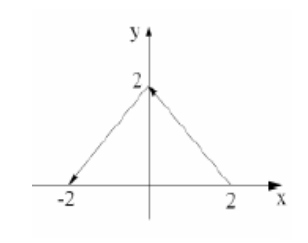
\includegraphics[scale = 1]{problema25.png}
	\caption{Gráfica del problema 25.}
\end{figure}

\vspace{5mm}

\noindent \textbf{Solución.}
\vspace{3mm}
El teorema de Green dice que 

\begin{align*}
	\oint_c P \di x + Q \di y = \iint \left( \frac{\partial Q}{\partial x} 
	- \frac{\partial P}{\partial y} \right) \di x \di y
\end{align*}

y como 
\begin{align*}
	\begin{cases}
		Q = 4xy^2 \implies 	\frac{\partial Q}{\partial x} = 4x \\ 
		P = y + 2x^2 \implies  \frac{\partial P}{\partial y} = 8xy	
	\end{cases}
\end{align*}

\begin{align*}
	W = \int_{-2}^{0} \int_0^{x+2} 4x -8xy \di y \di x 
	+ \int_0^2 \int_0^{-x+2} 4x-8xy \di y \di x
\end{align*}

El problema se divide en dos integrales debido a que dos funciones delimitan el área donde
se calcula la integral.

\begin{align*}
	W &= \int_{-2}^0 4x^2 + 8x - 4x^3 - 16x^2 -16x \di x + \int_0^2 -4x^2 + 8x -4 x^3 + 16x^2
	- 16x \di x \\
	& = 0 + 0 = \color{red} 0
\end{align*}
lo que nos dice el resultado es que el campo propuesto es conservativo, ya que una de las 
características de este tipo de campos es que la trayectoria no importa en el cálculo del
trabajo y, como en una curva cerra se empieza y termina en un mismo lugar, entonces
el trabajo es cero.

\vspace{5mm}

\noindent \textbf{Ejercicio 26:} Haciendo uso del teorema de Green, determinar el área del 
cardioide $x = a(2\cos t - \cos 2t)$, $y = (2\sen t - \sen 2t)$.
\vspace{5mm}

\vspace{3mm}
El teorema de Green dice que 

\begin{align*}
	\iint \left( \frac{\partial Q}{\partial x} 
	- \frac{\partial P}{\partial y} \right) \di x \di y =
	\oint_c P \di x + Q \di y  
\end{align*}

y como para calcular el área $\left( \frac{\partial Q}{\partial x} 
- \frac{\partial P}{\partial y} \right) = 1$, se puede escoger
arbitrariamente Q y P como
\begin{align*}
	Q = x && P = 0 &&\implies  &&A = \iint \left( \frac{\partial Q}{\partial x} 
	- \frac{\partial P}{\partial y} \right) \di x \di y = \int x \di y
\end{align*}
o
\begin{align*}
	Q = 0 && P = y &&\implies  &&A = \iint \left( \frac{\partial Q}{\partial x} 
	- \frac{\partial P}{\partial y} \right) \di x \di y = \int -y \di x
\end{align*}

Combinando los resultados anteriores se obtiene que 

\begin{align} \label{TeoGreen}
	A = \frac{1}{2}  \int x \di y + \int -y \di x
\end{align}

Ahora, obteniendo $x$, $\di x$, $y$ y $\di y$ se tiene que 
\begin{align*}
	&\begin{cases}
		x = 2a \cos t - a \cos 2t \\
		\di x = (-2a)(\sen t - \sen 2t) \di t
	\end{cases} \\
	&\begin{cases}
		y = 2 \sen t - \sen 25p \\
		dy = (2\cos t - 2\cos 2t)\di t
	\end{cases}
\end{align*}
Sustituyendo en \ref{TeoGreen} se llega a que 
\begin{multline*}
	A = \frac{1}{2} \int_0^{2\pi} -\left(2 \sen t - \sen 2t \right)\left(-2a
	\right)\left(\sen t - \sen 2t\right)
	+\\ \left(2a \cos t - a\cos 2t \right)\left(2 \cos t - 2 \cos 2t\right) \di t	
\end{multline*}
Desarrollando
\begin{multline*}
	A = \frac{1}{2} \int_0^{2\pi} 4a \sen^2 t - 6a \sen t \sen 2t + 2a \sen^2 2t +\\
	4a \cos^2 t - 6a \cos t \cos 2t + 2a \cos^2 2t \di t
\end{multline*}
Agrupando términos semejantes

\begin{align*}
	A = \frac{1}{2} \int_0^{2\pi} 6a (1-  \sen t\sen 2t + \cos t \cos 2t) \di t
\end{align*}

Aplicando la identidad del ángulo doble a $\sen 2t$ y a $\cos 2t$ y simplificando

\begin{align*}
	 A \footnotemark = \frac{1}{2} \int_0^{2\pi} 6a(1-\cos t) \di t = \color{red} 6a\pi u^2 
\end{align*} 
\footnotetext{El resultado difiere con el proporcionado en la serie, pero no se encontró 
forma de llenar a él. Además, obteniendo el área de un caso específico, el resultado
es más cercano al presentado aquí.}



\noindent \textbf{Ejercicio 27:} Utilizar el Teorema de Green para calcular el área de la región cerrada que es limitada por la elipse de ecuación $9x^2 + 4y^2 = 36$.

\vspace{5mm}

\noindent \textbf{Solución.}

\vspace{3mm}

\noindent Se sabe que calcular el área por integral doble equivale a integrar la función $f(x, y) = 1$. De esta forma, el integrando puede trabajarse como:

\begin{equation}\label{eqn:27-1}\tag{1}
	f(x, y) = \frac{\partial Q}{\partial x} - \frac{\partial P}{\partial y} \implies 1 = 1 - 0
\end{equation}

\noindent De la ecuación \eqref{eqn:27-1} obtenemos que $Q_x = 1$ y $P_y = 0$. Estas funciones se calculan a partir de la integración:

\begin{align*}
	Q_x = 1 \implies \int Q_x\, \mathrm{d}x = \int \mathrm{d}x \implies Q = x + C_1 \\
	P_y = 0 \implies \int P_y\, \mathrm{d}y = \int 0\, \mathrm{d}y \implies P = C_2 \\
\end{align*}

\noindent Como $C_1$ y $C_2$ son constantes arbitrarias, para el cálculo del área asumiremos que ambas son 0. Por lo tanto, la integral de línea a calcular es:

\begin{align*}
	\iint_R\,\mathrm{d}A = \oint_C\, P\,\mathrm{d}x + Q\,\mathrm{d}y = \oint_C\, x\, \mathrm{d}y
\end{align*}

\noindent Ahora debemos parametrizar la elipse dada, por lo que reescribimos la ecuación de forma estándar y posteriormente parametrizamos:

\begin{align*}
	9x^2 + 4y^2 = 36 \implies \frac{9x^2 + 4y^2}{36} = \frac{36}{36} \implies \frac{x^2}{4} + \frac{y^2}{9} = 1
\end{align*}

\begin{align*}
	\implies \begin{cases}
		x = 2\cos(t) \implies \mathrm{d}x = -2\sen(t)\\
		y = 3\sen(t) \implies \mathrm{d}y = 3\cos(t)\\
	\end{cases} \implies \underbrace{0 \leq t \leq 2\pi}_{\text{Se trata de una elipse cerrada.}}
\end{align*}

\noindent Procedemos a calcular la integral de línea a partir de la parametrización y los límites obtenidos:

\begin{align*}
	\oint_C\, x\,\mathrm{d}y = \Int_{0}^{2\pi}\, (2\cos t)(3\cos t)\,\mathrm{d}t = \Int_{0}^{2\pi}\, (6\cos^2 t)\,\mathrm{d}t
\end{align*}

\begin{align*}
	= 6\Int_{0}^{2\pi}\, \frac{1+\cos(2t)}{2},\mathrm{d}t
	\implies \frac{6}{2}\Int_{0}^{2\pi}\, 1+\cos(2t)\,\mathrm{d}t
\end{align*}

\begin{align*}
	= 3\,\left.\left(t + \frac{\sen(2t)}{2}\right)\right|_{0}^{2\pi} = 3\left[ \left(2\pi - 0\right) + \left( \cancelto{0}{\frac{\sen(4\pi)}{2}} - \cancelto{0}{\frac{\sen(0)}{2}} \right) \right] = 3(2\pi)
\end{align*}

\begin{align*}
	\pmb{\color{red} \therefore\: A = 6\pi\: \: u^2}
\end{align*}

\end{document}

 
